%\documentclass[paper]{ieicej}
%\documentclass[survey]{ieicej}% サーベイ論文
\documentclass[technicalreport]{ieicej} %今回のサーベイ論文の形式(多分)
%\documentclass[comment]{ieicej}% 解説論文
%\usepackage[dvips]{graphicx}
%\usepackage[dvipdfmx]{graphicx,xcolor}
\usepackage[fleqn]{amsmath}
\usepackage{newtxtext}% 英数字フォントの設定を変更しないでください
\usepackage[varg]{newtxmath}% % 英数字フォントの設定を変更しないでください
\usepackage{latexsym}
\usepackage[dvipdfmx]{graphicx}
%\usepackage{amssymb}

\setcounter{page}{1}

\field{A}
\jtitle{PUFに関する研究の調査と考察}
\etitle{}
\authorlist{
 \authorentry[okano.maiko.ol0@is.naist.jp]{岡野 舞子}{Maiko Okano}{NAIST}\MembershipNumber{2111062?}
 %以降,先輩方の名前を追加
}
\affiliate[NAIST]{奈良先端科学技術大学院大学
\hskip1zw 〒630–0192 奈良県生駒市高山町8916–5}{
  Nara Institute of Science and Technology, 8916–5 Takayama-cho, Ikoma, Nara, Japan
}
%\affiliate[所属ラベル]{和文所属}{英文所属}
%\paffiliate[]{}
%\paffiliate[現在の所属ラベル]{和文所属}
\jalcdoi{???????????}% ← このままにしておいてください

\begin{document}
\begin{abstract}
  フィジカリー・アンクローナブル・ファンクション(PUF)とは,主に半導体技術を用いて作られた集積回路を大量生産した際に生じる,制御不能な製造ばらつき
  を利用してその個体にランダムな関数を作る技術のことである.この技術は,個体の識別に用いることで模造品の作成を防ぐだけでなく,制御不能な性質を利用することで
  暗号アルゴリズムに組み合わせて使うことも期待されている.本稿ではPUFについて調査した内容を,その発展の歴史を踏まえて述べる.
  (全部書き終えたら,ちゃんと書き直す)
\end{abstract}
\begin{keyword}
  %和文キーワード 4〜5語
  PUF,真贋判定,認証,モデリング攻撃
\end{keyword}
\begin{eabstract}
  %英文アブストラクト 100 words
\end{eabstract}
\begin{ekeyword}
  %英文キーワード
  Physically Unclonable Function,Identification,Authentification,Modeling attack
\end{ekeyword}
\maketitle

\section{はじめに}
Internet of Things(IoT)の普及に伴い,現在,膨大な数のIoT機器がデータを収集し通信を行っている.
IoT機器の発展がもたらすSociety 5.0の実現は人々に便利さをもたらす一方,セキュリティリスクの増大が深刻な問題となっている.
この問題の一因として,製造品の偽造が挙げられる.
特に半導体産業は新型コロナウイルス流行の影響で工場が一部閉鎖されるなど打撃を受けたため,半導体不足により多くの偽造ICチップが出回っている\cite{ICfake}.
偽造ICチップは正規品よりも早く故障する可能性が高く,搭載されている機器の寿命を短くする恐れがある.
それだけでなく偽造品は誤作動を引き起こす可能性があるため,万が一重要なインフラで使用するIoT機器に偽造ICチップが使用されていた場合,
システム障害や情報漏えいといったセキュリティインシデントを引き起こす可能性がある.
したがってセキュリティ上の観点から,偽造ICチップの流通を防止する必要がある.

ICチップが正規品か偽造品か見分ける方法として,Physically Unclonable Function(PUF)を用いることが可能である.
PUFとは,大量生産された製造物(多くの場合,半導体技術を用いて作られたチップ)の製造時に生じる製造ばらつきを利用して,ランダムに各個体に付与された個性,またそれを利用した技術のことを指す.
この個性は製造者がプログラムやシリアル番号などを書き込むことなく,自動的に付与されるものであり同時に制御不能なものである.
したがって,その個性をもった個体のクローンを作成することを防ぎ,人間を指紋や虹彩で識別するように製造物の個体識別が可能となる.

従来,シリアル番号が製造物の個体識別や品質管理に用いられていたが,シリアル番号とPUFの最も異なる点はクローンの製造が可能か否かである.
シリアル番号はただの文字列であるため,悪意のある攻撃者に一度認識されれば偽造品の製造を避けることは難しい.
しかし,PUFは製造時の制御不能なばらつきを利用してIDを作成するため,同じPUFの製造物を偽造することは対象の製品の微小な個体差までを
完璧に再現することに等しく,非常に困難である.

また,PUFは製造品の個体識別だけでなく,認証や秘密鍵の管理に使うことができると考えられている.
秘密鍵の管理は従来であれば不揮発性メモリで行っていたが,不揮発性メモリはチップを開封して解析を行う静的リバース・エンジニアリングに耐性がない.
しかしPUFを用いた鍵管理は,動作時にしか鍵が顕在しないためそのような攻撃に耐性がある.

PUFはハードウェアセキュリティの要素の1つとして盛んに研究されており,また企業や研究機関によって実用化されつつある.
そのため,本稿はPUFの特性や主流となる構造を理解し,それによってPUFにどのような脆弱性があるかを考察を行うのを目的としている.
\ref{puf}章ではPUFの特性や考えられている活用法について述べる.
\ref{pufhis}章ではPUFの起源へと遡り,PUFの歴史をふまえつつ構築法について説明する.
また,PUFの強度による分類とそれに伴うPUFの使用法としての種類について述べる.
\ref{pufpro}章ではそれまでの内容を踏まえ,PUFへの攻撃法を紹介する.
\section{Physically Unclonable Function}
\label{puf}
\subsection{PUFの定義}
PUFの意味を,PUFの名前に沿って説明する.
\begin{description}
  \item[\textbf{Physically}]物理的な特徴を有していること.製造者は同一の設計図から大量の個体を製造し,その際に生じる製造ばらつきにより個体ごとの違いが生じる.
  \item[\textbf{Unclonable}]上記の物理的な個性は,複製不可能である.また,個性と個体は切り離すことができず,別の個体にその個性を付与することはできない.
  \item[\textbf{Function}]PUFはチャレンジとして外部から刺激を与えられたとき,レスポンスとして測定値を出力する.つまり,関数である.
\end{description}


制御不能な製造ばらつきを利用するため,同じPUFに同じチャレンジを入力してもレスポンスは多少異なる.
しかし,同じレスポンスを異なるPUF個体に入力したとき,出力されるレスポンスは区別可能なほどに異なるため,これがランダム関数の機能を果たす.

また,チャレンジと,それをPUFに入力して出力されたレスポンスのペアをチャレンジ・レスポンス・ペア(CRP)と呼ぶ.
\subsection{PUFに求められる特性}
本節では,PUFに求められるセキュリティに関する特性を説明する.
要求される重要な特性の説明を通して,実際のPUFがどのような機能を果たすかの理解を深めることが狙いである.
しかし,本稿執筆時点(2021年7月2日)でPUFのセキュリティ要件及び試験方法は,ISO/IEC 20879にて議論中となっている.
そのため,ここでの内容は主に菅原\cite{sugatake}とMaes\cite{maes1}に基づいている.

%まず,再現性・ユニーク性・耐クローン性の3つの特性について述べる.
%この3つの特性は,PUFの機能の根幹を支えるとりわけ重要な特性である.
本稿ではPUFの機能の根幹を支える,とりわけ重要な3つの特性(再現性・ユニーク性・耐クローン性)について述べる.
\subsubsection{再現性(Reproducibility)}
再現性とは,同一のPUFに同じチャレンジを繰り返し入力したとき,出力されるレスポンスのばらつきの小ささ,
つまり安定度の高さを表す.PUFのレスポンスにはノイズが含まれており,同じ個体に同じチャレンジを入力しても
出力されるレスポンスには差異が生じる.PUFの実用の観点から,同じ個体からのレスポンスは類似している必要があるため,
再現性は高いほうが良い.

再現性は,同一チップのPUF出力ビット列のハミング距離(Hamming Distance: HD),Intra-HDを評価指標としている.
このとき,Intra-HDの平均の理想値は0である.
また,この指標は,PUFのノイズの大きさを測るだけでなく,環境変化の影響を評価する場合にも用いる.
\subsubsection{ユニーク性(Uniqueness)}
ユニーク性とは,異なるPUFに同一のチャレンジを入力したとき,出力されるレスポンスの値の差の大きさを表す.異なるPUFのレスポンスの
値の差が小さい(類似している)場合,それらを同一であると誤判定してしまう可能性が高まる.そのため,
PUFの個体差,つまりユニーク性は高いほうがよい.

ユニーク性は,異なるチップのPUF出力ビット列のハミング距離,Inter-HDを評価指標としている.
このとき,Inter-HDの平均の理想値は0.5であり,この値に近いほどユニーク性は高い.
\subsubsection{耐クローン性(Unclonable)}
耐クローン性とは,PUFのチャレンジに対するレスポンスを再現するモデルの構築が不可能,あるいは困難であることを
表している.PUFを利用してある個体と別の個体を識別するためには,ある個体を模したクローンを作成できないという
前提条件が必要である.

この特性には2つの意味があり,1つは正規製造者であってもクローンを作ることができないこと(=製造者耐性),
もう1つはクローンの制作を試みる攻撃への耐性を持つ(クローンを作るための既知の攻撃が存在しない)ことである.
\subsection{PUFの活用法}
\label{puf use}
\subsubsection{真贋判定・個体識別}
PUFのCRPが完全に同じになるPUFは2つと存在しないため,個体を識別することが可能である.
このとき,チャレンジ・レスポンス認証を行うことで,PUFの認証を行う.

認証とは,通信において相手が本人か否かを確認する技術である.
暗号を用いた認証では,認証する側と認証される側が,あらかじめ交換しておいて秘密鍵をもっているかどうか確かめることで行う.
このとき秘密鍵を露出することなく認証を行う手段にチャレンジ・レスポンス認証がある.

この認証方式では共通鍵暗号アルゴリズムを用いるが,ここではそれをPUFで代用する.
しかし,認証のためには認証者と被認証者が同じ関数を共有する必要があるが,PUFは複製不可能であるため2者が同一の関数を持つことができない.
この問題を解決するために,CRPのリストをあらかじめ作成し,それを認証者が保管する方法がある.
このCRPリストの保管は,PUFを搭載した製品を出荷する際,メーカーが工場などで実行することが想定される.
そして,認証時には被認証者が送信したレスポンスが,事前に作成されたリストに登録されているか確かめることで,
相手が正しいか(正規品か)どうかを判別する.
\subsubsection{鍵の生成}

\section{様々なPUF}
\label{pufhis}
\subsection{PUFの歴史と構築法}
\subsubsection{初期のPUF}
\label{firstpuf}
\paragraph{Physical one-way functions}
PUFの始祖とされているのは,2001年にPappuが提案した物理的一方向性関数(Physical one-way functions: POWF)\cite{pappu}である.
背景としては,既存の数論に基づいた一方向性関数の課題に対する解決策として提案された.
POWFの簡略化した手順を以下に示す.
\begin{enumerate}
  \item 3次元の不規則な構造の媒体をトークンとして用意する.具体的には,極小のガラス玉をいくつか含んだエポキシ樹脂とされている.
  \item 上記の媒体にレーザー光を照射したものを,電化結合素子カメラで記録する.これによって,2次元のスペックルパターンを得る.
  \item スペックルパターンをガボール変換でフィルタリングし,鍵となるビット列(1次元)を生成する.
\end{enumerate}

\paragraph{Silicon PUF}
\label{SiliconPUF}
POWFは精密な光学機器で処理を行う必要があるため,アナログインターフェイスで使用するように作られている.
一方でGassendは2002年に,計算機やメモリと混載できるようにデジタルインターフェイスで動作する,半導体製のPUF(Silicon PUF)を提案した\cite{gassend1}.
Sillicon PUFは前述のPOWFと異なり,暗号実装のハードウェア構成要素としてすぐに導入することができるため,
現在研究されているPUF構築の主要な種類となっている.

Gassendが提案したPUF\cite{gassend1}の構成は,\ref{ROPUF}節のRing Ocillator PUFの起源となっている.
このPUFは,各回路の遅延のばらつきを利用し,過渡応答を測定することでCRPsを生成する.
過渡応答は,チャレンジによって刺激された経路上にあるIC内の配線やデバイスの遅延についての間接的な情報となる.
この間接的な情報しかレスポンスとして与えられないことが,耐クローン性の根拠となっている.

また,“PUF”という名前やPUFの定義が明記されたのは,この論文が最初である.

\subsubsection{遅延ベースのPUF}
\label{delaypuf}
\paragraph{Arbiter PUF}
\label{apuf}
\ref{firstpuf}節\ref{SiliconPUF}のGassendが提案したPUFは,回路の遅延が温度や電源電圧などの環境変化に敏感であるため,
PUFの信頼性を高めるためにはノイズが重大な問題となる,とLeeは指摘を行った\cite{lee}.
そこでLimらは2004年にSillicon PUFの再現性を改善させたArbiter PUF\cite{lim}を実装した.
Arbiter PUFは差動構造(Arbiter)に基づいており,環境に起因するノイズに対するPUFの再現性を向上させることが可能である.
これは,PUFのレスポンスに対する絶対的な遅延値を測定する代わりに,2つの同一の遅延経路を比較し,
Arbiterを用いてデジタル情報を生成するためである.

%ここでアービターPUFの図を入れたい\label{APUF}
\begin{figure}[tb]
  \begin{center}
    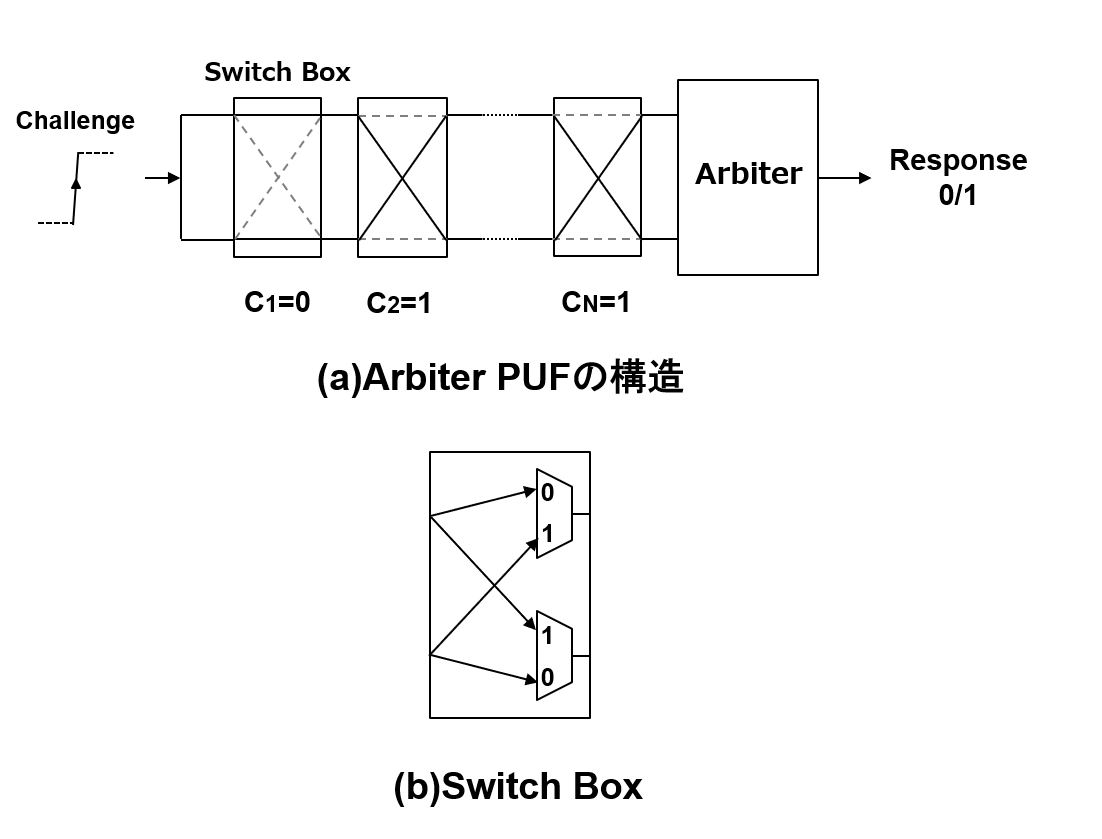
\includegraphics[width=75mm]{Apuf.png}
  \end{center}
  \caption{Arbiter PUFの構築法}
  \label{APUF}
\end{figure}
%前半,後半で分ける余裕があるかはわからん
Arbiter PUFの構造は前半と後半に分けられる.
最初に2つの入力から立ち上がり信号(=チャレンジ)が同時に入力され,
前半部ではチャレンジによって,2つの信号がどのような経路を伝搬するかが決定される.
図\ref{APUF}のとおり2つのMUXによってスイッチボックスが実装されており,これはチャレンジのビット数の分用意される.
スイッチボックスの動作は,チャレンジのビットが1のときは上下に流れる信号の経路を交差,0のときは直進となっている.

後半部では,1つのトランスペアレントラッチが使用されており,どちらの信号が先に到達したかによって0か1のレスポンスを出力する.
%ここでは1つのトランスペアレントラッチが使用されており,これは表\ref{apuf-transparent}が示すような動作を行う.
%表\label{apuf-tranparent}
%\begin{table}[tb]
%  \caption{和文キャプション}
%  \label{apuf-transparent}
%\ecaption{英文キャプション}
%  \begin{center}
%    \begin{tabular}{|l|l|l|}
%      \Hline %% ←
%      \multicolumn{2}{|c|}{\textbf{Inputs}} & \multicolumn{1}{c|}{\textbf{Outputs}}              \\
%      \hline
%      \textbf{G}                            & \textbf{D}                            & \textbf{Q} \\
%      \hline
%      0                                     & 0                                     & 0          \\
%      \hline
%      0                                     & 1                                     & 1          \\
%      \hline
%      1                                     & X                                     & No Change  \\
%      \hline
%      $\uparrow$                            & D                                     & d          \\
%      \Hline %% ←
%    \end{tabular}
%  \end{center}
%\end{table}
%2つの立ち上がり信号が違うタイミングでDとGに入力された場合,Gに立ち上がり信号が入力された瞬間のDの値を常に出力し続ける.
%つまり,Dに先に立ち上がり信号が到達した場合,その後Gに立ち上がり信号が到達することを意味するため,レスポンスは1となる.
%逆にGに先に立ち上がり信号が到達した場合は,その時点でのDには0が入力されていることからレスポンスは0となる.

\paragraph{Ring Oscillator PUF}
\label{ROPUF}
2007年にSuhによって提案されたRing Oscillator PUF(RO PUF)\cite{suh}は,ROの発振周波数が製造ばらつきによって異なることを基にしたPUFである.
ROは奇数個のインバータから構成されている.
\begin{figure}[tb]
  \begin{center}
    
\includegraphics[width=75mm]{ROpuf.png}
  \end{center}
  \caption{RO PUFの構築法}
  \label{ROPUF-fig}
\end{figure}
奇数個のインバータをループ上に並べ(図\ref{ROPUF-fig}(b)),その中のある一点の値を出力に利用することでROの出力は一定の周期で0と1を繰り返す.
インバータの個数や配線方法などがまったく同じROであっても,回路内部の部品の製造ばらつきによって微妙に発振周波数が異なり,
RO PUFではこの発振周波数の違いを用いてPUFの機能を提供する.
RO PUFでは3個以上のROが用いられており,その中からチャレンジの値によって2つのROを選出する.
そしてその2つのROの周波数の比較によってレスポンスとなる0か1のビットを出力する.

図\ref{ROPUF-fig}(a)のように複数(この場合は$N$個)のROはMUXに接続され,チャレンジはそのMUXのセレクタとして用いられる.
セレクタにより選ばれた2つの信号はそれぞれ別のカウンター回路に入力しており,カウンター回路で計測された一定時間あたりの
発振回数が比較されその結果によってRO PUFから0か1の値が出力される.
\subsubsection{メモリベースのPUF}
\label{memorypuf}
\paragraph{SRAM PUF}
\label{SRAM PUF}
SRAM PUFとは,電源投入直後にまだ何も書き込んでいないSRAMから読みだした値(初期値)を個体差として利用するPUFである\cite{sugatake}.
2006年にSimpsonによって,PUFを利用してFPGAのIP保護を行うというアプローチ\cite{simpson}が提案された.
この提案を元に,2007年にGuajardoはFPGAに搭載されているSRAMをPUFとして実装\cite{guajaudo}した.
また,同時期の類似研究としてHolcombのFERNS(Fingerprint Extravtion and Random Numbers in SRAM)\cite{holcomb}がある.
FERNSはSRAM PUFと非常に類似しているが,市販のSRAMチップとマイクロコントローラチップに組み込まれたSRAMという
2つの異なるプラットフォームで実装がされている点で,Guajaudoの研究とは異なっている\cite{maes1}.

SRAM PUFの動作原理は,SRAMセルの電源投入時の過渡的な動作に基づいている.
電源投入直後,セルは動作点が定まらず不安定な状態となるが,ごく短時間のうちに動作点は定まり安定する.
この初期の動作点(初期値)は,電源投入時,毎回高い確率で同じになる.
何故なら,製造ばらつきによってトランジスタに僅かな電圧差が生じるため,クロスカップリングされたインバータ回路の
MOSFETの「強さ」に違いが出るためである\cite{maes1}.
したがって,各SRAMセルはランダムに0と1のいずれかに遷移していくため,これがPUFのユニーク性の根拠となる.
また,チャレンジはSRAM内の特定のセルのアドレスである.
\paragraph{Butterfly PUF}
2008年にKumarらは,起動時にSRAMセルと同様の動作をする構造をFPGAマトリクス内に実装し,これをButterfly PUF\cite{kumar}として提案した.
これはほとんどの市販FPGAに搭載されているSRAMは,電源投入直後に強制的にクリアされるため,
\ref{SRAM PUF}節で説明したセルごとのランダムな初期値をPUFとして利用することができないからである.

Butterfly PUFの実装は,2つの透過的なデータラッチを交差結合し,SRAMセルの動作をFPGAのリコンフィギュレーションロジックで模倣することで行われる.
ラッチを使って交差結合構造を作り,これにより励起状態によって不安定な状態となる.
そして,しばらくすると2種類の安定状態のうちの1つに落ち着くため,これがPUFのレスポンスとなる.
\subsubsection{その他の特徴を持つPUF}

\subsection{PUFの分類}
\subsubsection{Strong/Weak PUF}
PUFは,CRPの空間の広さによってStrong PUFとWeak PUFの2つに分けられる.

Strong PUFはCRPの空間が極めて広いPUFであり,チャレンジ長が増大するとCRP空間が指数関数的に増大する.
また十分に長いチャレンジを与えることができる,という特徴をもつ.
例としてはArbiter PUFが挙げられる.
スイッチボックスの個数が$n$個の場合チャレンジ数は$2^n$個となるため,$n=128$のときペア数は$2^{128}$となり
CRPを全通り試すことは困難になる.

Weak PUFはCRP空間が狭いPUFであり,物理的な制約によって十分なチャレンジ長を確保することができないPUFである.
例としてSRAM PUFが挙げられる.
SRAM PUFは搭載できるメモリ素子の数に限りがあるので,チャレンジ長は高々アドレス長までとなる.
典型的なSRAMのサイズは数キロバイトから数メガバイトであり,SRAM PUFを全探索攻撃から防ぐことは困難である.

ところで,Strong/Weak PUFの"Strong/Weak"はPUFの実利用におけるセキュリティ強度とは,直接結びつかないことに注意する必要がある.
例として,PUFを製品の真贋鑑定の認証として用いるか,セキュリティパラメータの生成として用いるかでは,求められるCRP空間の広さは異なる.
現在,Strong/Weakの名前はしばしば誤解を生じさせることがあるので,ISO/IEC 29897で別の名称(Extensive/Confined)が提案されている\cite{hori-nedo}.

\subsubsection{Controlled/Uncontrolled PUF}
Controlled PUFとは,特定のAPIでしかアクセスできないようにアルゴリズムで制御されたPUFである\cite{gassend-cpuf1}\cite{gassend-cpuf2}.
逆にPUFへのアクセス制御がなく,誰でもPUFの生の入出力にアクセスできる場合は,Uncontrolled PUFと呼ぶ.

Uncontrolled PUFはシンプルな利用法であり,アクセス制御のためのデジタル回路が不要であることから,
回路をより小型にすることができるという利点がある\cite{sugatake}.
しかし,攻撃者はありうるすべてのチャレンジをPUFに入力することで,対応するレスポンスを入手して対応表を作るクローン攻撃が可能となる.
このような攻撃に対しUncontrolled PUFは,CRPを全探索できないほど大きくする方法でしか対策を行えない.

Controlled PUFはPUFの生データを秘匿するため,攻撃者にCRPsを知られることを防ぎモデリング解析の対策になると考えられている.
そのため,SRAM PUFなどのWeak PUFはControlled PUFとして実装されることが望ましい.

\section{PUFの問題}
\label{pufpro}
\subsection{PUFへの攻撃}
\subsubsection{モデリング攻撃}
モデリング攻撃とは,PUFからCRPsやサイドチャネルなどの情報を取得して,それを用いてPUFのクローンとなる関数を生成する攻撃である.
\ref{puf use}節で紹介したようにPUFをセキュリティの要素として使うためには,あるチャレンジに対応するレスポンスが推定されないことが重要である.

\ref{delaypuf}節\ref{apuf}のArbiter PUFは導入当初から,モデリング攻撃を受けやすいことが認識されていた\cite{maes1}\cite{lim}.
これは,PUFの再現性を高めるためにArbiter PUFのチャレンジとレスポンスの間の依存関係の複雑さが軽減されたためである.
とはいえ,Arbiter PUF以外のPUFも機械学習の発展により,モデリング攻撃の研究が多数存在する.

モデリング攻撃はPUFに対する攻撃として最も主流であり,現在に至るまで多くの結果が報告されている.
今回,モデリング攻撃をするにあたってどのPUF情報を利用したかによって,モデリング攻撃の分類を行う.
\paragraph{CRPsの取得による攻撃}
\label{Crps}
取得したCRPsを機械学習を用いて学習することで,PUFの近似となる関数を取得する攻撃である.
\ref{sidechannel},\ref{reattack}節で紹介する攻撃手法と違い,電磁波を測定する装置や対象の機器に接触する必要がないため,
解析難易度は比較的低いと考えられている\cite{nozaki}.
したがって,モデリング攻撃の中ではこの攻撃手法が主流であると考えられる.

調査したところ,この攻撃手法の対象となるPUFはArbiter PUF\cite{crps apuf1,crps apuf2,crps apuf3 multi1,crps apuf4 side,crps apuf5 multi2,crps apuf6,crps modeling,crps apuf7 crc}
とRO PUF\cite{nozaki,crps modeling,crps RO}
をベースにしたPUFに多く確認した.
これは,これらのPUFは一般的な使い方ではStrong PUFに分類され,CRPsの空間が広くUncontrolled PUFとして使用されるため
機械学習を行いやすいためであると考えられる.
また,機械学習アルゴリズムの発展により,少ないCRPsでモデリング攻撃を行う研究もなされている\cite{nozaki}.
対策としては,Strong PUFに機械学習によるクローン生成が難しいWeak PUFを組み合わせたマルチPUF\cite{crps apuf3 multi1,crps apuf5 multi2}や改良されたPUF\cite{crps apuf7 crc}を構築することで
CRPsの規則性をなくすアプローチがとられている.

\paragraph{サイドチャネル情報による攻撃}
\label{sidechannel}
攻撃者は消費電力や漏洩する電磁波を観測することでPUF内部の情報を取得し,それを基にモデリング攻撃を行うことも可能である.

Controlled Arbiter PUFは\ref{Crps}のようなCRPsの機械学習による攻撃には耐性があると考えられているが,
消費電力を測定することで得た情報を元に機械学習することでモデリング攻撃が可能であると指摘されている\cite{side apuf}.
また,RO PUFの漏洩電磁波を用いた手法\cite{side rpuf1,side rpuf2,side rpuf3}もいくつか提案されている.
\subsubsection{リバース・エンジニアリングによる攻撃}
\label{reattack}
PUFは電源投入後にしか鍵が顕在しないため,電源オフ時に行う静的リバース・エンジニアリングに耐性がある.
しかし,


\section{まとめ}

%\ack %% 謝辞

%\bibliographystyle{sieicej}
%\bibliography{myrefs}
\begin{thebibliography}{99}% 文献数が10未満の時 {9}
  \bibitem{ICfake}
  Gigazine,“世界的な半導体不足によって偽造チップが広がっている,”
  https://gigazine.net/news/20210615-chip-shortages-lead-counterfeit/,
  参照 July 18, 2021.
  \bibitem{sugatake}
  菅原健,“暗号ハードウェアの研究開発動向:フィジカリー・アンクローナブル・ファンクション,”
  金融研究,vol.39,no.4,pp.25-54,Oct. 2020.
  \bibitem{maes1}
  R. Maes, Physically Unclonable Functions: Properties, Springer, Berlin, Heidelbelg, 2013.
  (DOI:10.1007/978-3-642-41395-7\_3)
  \bibitem{pappu}
  P.S. Ravikanth, “Physical One-Way Functions,” PhD thesis,
  Massachusetts Institute of Technology, March 2001.
  %\bibitem{gassend2}

  \bibitem{gassend1}
  B. Gassend, D. Clarke, M. van Dijk, S. Devadas, “Silicon physical random funcions,”
  CCS '02: Proceedings of the 9th ACM conference on Computer and communications security,
  pp.148-160, November 2002. (DOI: 10.1145/586110.586132)
  \bibitem{lee}
  J.W. Lee, D. Lim, B. Gassend, G.E. Suh, M. van Dijk, S. Devadas,
  “A Technique to Build a Secret Key in Integrated Circuits for Identification and Authentication Applications,”
  2004 Symposium on VLSI Circuits. Digest of Technical Papers (IEEE Cat. No.04CH37525),
  pp. 176-179, June 2004. (DOI: 10.1109/VLSIC.2004.1346548)
  %\bibitem{lim}
  %D. Lim, J.W. Lee, B. Gassend, G.E. Suh, M. van Dijk, S.Devadas,
  %“Extracting secret keys from integrated circuits,” IEEE Tran. Very Large Scale Integration (VLSI) Systems,
  %vol.13, no.10, pp.1200-1205, Oct. 2005.(DOI: 10.1109/TVLSI.2005.859470)
  \bibitem{lim}
  D. Lim, “Extracting Secret Keys from Integrated Circuits,” Master's Thesis,
  Massachusetts Institute of Technology, March 2004.
  \bibitem{suh}
  G.E. Suh, S. Devadas,“Physical Unclonable Functions for Device Authentication and Secret Key Generation,”
  2007 44th ACM/IEEE Design Automation Conference, pp.9-14, June 2007.
  \bibitem{simpson}
  E. Simpson, P. Schaumont, Offline Hardware/Software Authentication for Reconfigurable Platforms.
  In: Goubin L., Matsui M. (eds) Cryptographic Hardware and Embedded Systems - CHES 2006.
  CHES 2006. Lecture Notes in Computer Science, vol 4249, Springer, Berlin, Heidelberg, 2006.
  (DOI: 10.1007/11894063\_25)
  \bibitem{guajaudo}
  J. Guajardo, S.S. Kumar, GJ. Schrijen, P. Tuyls, FPGA Intrinsic PUFs and Their Use for IP Protection,
  Proceedings of International Workshop on Cryptographic Hardware and Embedded Systems (CHES) 2007,
  Lecture Notes in ComputerScience, vol 4727, Springer-Verlag, pp. 63–80, 2007.
  (DOI: 10.1007/978-3-540-74735-2\_5)
  \bibitem{holcomb}
  D. E. Holcomb, W. P. Burleson , K. Fu,
  "Power-Up SRAM State as an Identifying Fingerprint and Source of True Random Numbers,"
  in IEEE Transactions on Computers, vol. 58, no. 9, pp. 1198-1210, Sept. 2009.
  (DOI: 10.1109/TC.2008.212.)

  \bibitem{hori-nedo}
  堀洋平,“Physically Unclonable Function(PUF)の基礎,応用と標準化について,” https://www.iot-aidevice.org/app/download/14287213\\
  230/AI2oT3\_堀\_+PUFの基礎\_応用と標準化.pdf?t=1548407303,
  参照July 16, 2021.
  \bibitem{gassend-cpuf1}
  B. Gassend, D. Clarke, M. van Dijk and S. Devadas, "Controlled physical random functions,"
  18th Annual Computer Security Applications Conference, 2002. Proceedings.,
  pp. 149-160, Nov. 2002. (Doi: 10.1109/CSAC.2002.1176287)
  \bibitem{gassend-cpuf2}
  B. Gassend, M. van Dijk, D.Clarke, E.Torlak, S. Devadas, P.Tuyls,
  "Controlled physical random functions and applications,"
  ACM Transactions on Information and System Security, Volume 10, Issue 4, Article No.3, pp 1–22,
  Jan. 2008.(DOI:10.1145/1284680.1284683)
  \bibitem{kumar}
  S.S. Kumar, J. Guajardo, R. Maes, G. Schrijen, P. Tuyls,
  "Extended abstract: The butterfly PUF protecting IP on every FPGA,"
  2008 IEEE International Workshop on Hardware-Oriented Security and Trust, pp.67-70,
  June 2008.(DOI: 10.1109/HST.2008.4559053)

  \bibitem{nozaki}
  野崎佑典, 梅田大知, 竹本修, 吉川雅弥,
  “リングオシレータPUFに対する遺伝的アルゴリズムを用いたハイブリッドモデリング解析とその評価,”
  電気学会論文誌C(電子・情報・システム部門誌), 140 巻, 12 号, p. 1307-1315, Dec. 2020.
  (DOI: 10.1541/ieejeiss.140.130)
  %crps modeling attack
  \bibitem{crps modeling}
  U. Rührmair et al., "PUF Modeling Attacks on Simulated and Silicon Data,"
  in IEEE Transactions on Information Forensics and Security, vol. 8, no. 11, pp. 1876-1891, Nov. 2013.
  doi: 10.1109/TIFS.2013.2279798.
  \bibitem{crps apuf1}
  J. Ye, Y. Hu and X. Li, “RPUF: Physical Unclonable Function with Randomized Challenge to resist modeling attack,”
  2016 IEEE Asian Hardware-Oriented Security and Trust (AsianHOST), pp. 1-6, Dec. 2016.
  (Doi: 10.1109/AsianHOST.2016.7835567)
  \bibitem{crps apuf2}
  C. Gu, C. H. Chang, W. Liu, S. Yu, Q. Ma and M. O'neill,
  “A Modeling Attack Resistant Deception Technique for Securing PUF based Authentication,”
  2019 Asian Hardware Oriented Security and Trust Symposium (AsianHOST), pp. 1-6, Dec. 2019.
  (Doi: 10.1109/AsianHOST47458.2019.9006710)
  \bibitem{crps apuf3 multi1}
  Q. Ma, C. Gu, N. Hanley, C. Wang, W. Liu and M. O'Neill, “A machine learning attack resistant multi-PUF design on FPGA,”
  2018 23rd Asia and South Pacific Design Automation Conference (ASP-DAC), pp. 97-104, Jan. 2018.
  (doi: 10.1109/ASPDAC.2018.8297289)
  \bibitem{crps apuf4 side}
  T. Kroeger, W. Cheng, S. Guilley, J. -L. Danger and N. Karimi,
  "Effect of Aging on PUF Modeling Attacks based on Power Side-Channel Observations,"
  2020 Design, Automation \& Test in Europe Conference \& Exhibition (DATE), pp. 454-459, March 2020.
  doi: 10.23919/DATE48585.2020.9116428.
  \bibitem{crps apuf5 multi2}
  Y. Cui, C. Gu, Q. Ma, Y. Fang, C. Wang, M. O’Neill, and W. Liu, “Lightweight Modeling Attack-Resistant Multiplexer-Based Multi-PUF (MMPUF) Design on FPGA,”
  Electronics, vol. 9, no. 5, p. 815, May 2020.
  \bibitem{crps apuf6}
  M. Ebrahimabadi, M. Younis, W. Lalouani and N. Karimi, "A Novel Modeling-Attack Resilient Arbiter-PUF Design,"
  2021 34th International Conference on VLSI Design and 2021 20th International Conference on Embedded Systems (VLSID), pp. 123-128, Feb. 2021.
  doi: 10.1109/VLSID51830.2021.00026.
  \bibitem{crps apuf7 crc}
  E. Dubrova, O. Näslund, B. Degen, A. Gawell and Y. Yu, "CRC-PUF: A Machine Learning Attack Resistant Lightweight PUF Construction,"
  2019 IEEE European Symposium on Security and Privacy Workshops (EuroS\&PW), pp. 264-271, June 2019.
  doi: 10.1109/EuroSPW.2019.00036.
  \bibitem{crps RO}
  Q. Wang, M. Gao, and G. Qu, “A Machine Learning Attack Resistant Dual-mode PUF,”
  In Proceedings of the 2018 on Great Lakes Symposium on VLSI (GLSVLSI '18),
  Association for Computing Machinery, pp.177–182, May 2018.
  \bibitem{side apuf}
  G.T. Becker, R. Kumar,“Active and Passive Side-Channel Attacks on Delay Based PUF Designs,”
  IACR Cryptology ePrint Archive, vol. 2014, pp.287, 2014.
  \bibitem{side rpuf1}
  Y. Cao, X. Zhao, W. Ye, Q. Han, and X. Pan, “A Compact and Low Power RO PUF with High Resilience to the EM Side-Channel Attack and the SVM Modelling Attack of Wireless Sensor Networks,”
  Sensors, vol. 18, no. 2, p. 322, Jan. 2018.
  \bibitem{side rpuf2}
  M. Shiozaki, T. Fujino,
  “Simple electromagnetic analysis attack based on geometric leak on ASIC implementation of ring-oscillator PUF,”
  J Cryptogr Eng, Sep. 2020.
  \bibitem{side rpuf3}
  D. Merli, D. Schuster, F. Stumpf, G. Sigl,“Semi-invasive EM attack on FPGA RO PUFs and countermeasures,”
  Association for Computing Machinery, New York, NY, USA, 2011.
\end{thebibliography}

%\appendix
%\section{}

%\begin{biography}
% \profile{}{}{}
%\profile{会員種別}{名前}{紹介文}% 顔写真あり
%\profile*{会員種別}{名前}{紹介文}% 顔写真なし
%\end{biography}

\end{document}